\documentclass[french, 12pt]{report}
\usepackage[latin1, utf8]{inputenc}
\usepackage{color}
\usepackage{graphicx}
\usepackage{listings}
\usepackage{amssymb}
\usepackage{amsmath}
\usepackage{pstricks}
\usepackage{enumitem}
\usepackage{multicol}
\usepackage[paper=a4paper,margin=1in]{geometry}
\usepackage{verbatim}
\usepackage{listings}
\usepackage{tikz}
\usetikzlibrary{arrows,automata}
\usetikzlibrary{shapes,snakes}
\usepackage{pgfplots}
\usepackage{pgfplotstable}
\usepackage{xifthen}
\usepackage{fancyhdr}
\usepackage{caption}
 
% \pgfplotsset{compat=1.16}
\setlist[description]{leftmargin=\parindent,labelindent=\parindent}

\definecolor{gray}{rgb}{0.4,0.4,0.4}
\definecolor{darkblue}{rgb}{0.0,0.0,0.6}
\definecolor{cyan}{rgb}{0.0,0.6,0.6}
\definecolor{darkgreen}{RGB}{0,150,0}
 	
\newcommand{\cblue}[1]{ \textcolor{blue}{#1}}
\newcommand{\corange}[1]{ \textcolor{orange}{#1}}
\newcommand{\cviolet}[1]{ \textcolor{violet}{#1}}
\newcommand{\crouge}[1]{ \textcolor{red}{#1}}
\newcommand{\cvert}[1]{ \textcolor{darkgreen}{#1}}
\newcommand{\cgris}[1]{ \textcolor{gray}{#1}}

%% ------------------------- Header Footer
\pagestyle{fancy}
\fancyhf{}
\fancyhead[LE,RO]{Master 2 État de l'art}
\fancyhead[RE,LO]{ }
\fancyfoot[CE,CO]{\leftmark}
\fancyfoot[LE,RO]{\thepage}
% -------------------------- END Header Footer

%% ------------------------- Formular
\newcommand{\cformular}[2]{
\begin{center} 
\begin{description} 
\item[#1] #2 
\end{description} 
\end{center}
}
%% ------------------------- END Formular

%% ------------------------- RO Model
\newcommand{\rovarinout}[5]{
\begin{description}
\item[La variable entrante sera] #1
\item[La variable sortante sera] #2 car:
\end{description}
\begin{multicols}{3}
#3, #4, #5
\end{multicols}
}

\newcommand{\romodel}[8]{
\begin{multicols}{2}
[Voici le nouveau modèle:]
\begin{description}
\item[Déterminer] #1
\item[#2] #3 % ((2) maximisant | minimisant )
\item[Variables hors base] #4
\item[Variables de Base] #5
\item[Solution admissible] #6 et Z = #7
\end{description}
#8 % contraintes
\end{multicols}
}
%% ------------------------- END RO Model

%% ------------------------- XML

\lstset{
  basicstyle=\ttfamily,
  columns=fullflexible,
  showstringspaces=false,
  commentstyle=\color{gray}\upshape
}

\lstdefinelanguage{XML}
{
  morestring=[b]",
  morestring=[s]{>}{<},
  morecomment=[s]{<?}{?>},
  stringstyle=\color{black},
  identifierstyle=\color{darkblue},
  keywordstyle=\color{cyan},
  morekeywords={xmlns,version,type}% list your attributes here
}
%% ------------------------ END XML

%% ------------------------ Almost all
\newcommand{\almost}{\mid\kern-0.40em{\backsim}\ }
%% ------------------------ END Almost all

%% ------------------------ Inverse DL lite
\newcommand{\inverse}{\urcorner\ }
%% ------------------------ End Inverse DL lite

%% ------------------------ Python code for Machine leaning
\definecolor{codegreen}{rgb}{0,0.6,0}
\definecolor{codegray}{rgb}{0.5,0.5,0.5}
\definecolor{codepurple}{rgb}{0.58,0,0.82}
\definecolor{backcolor}{rgb}{0.97,0.97,0.95}

\lstdefinestyle{mlpythoncode}{
    backgroundcolor=\color{backcolor},   
    commentstyle=\color{codepurple},
    keywordstyle=\color{codegreen},
    numberstyle=\tiny\color{codegray},
    stringstyle=\color{magenta},
    basicstyle=\footnotesize,
    breakatwhitespace=false,         
    breaklines=true,                 
    captionpos=b,                    
    keepspaces=true,                 
    numbers=left,                    
    numbersep=5pt,                  
    showspaces=false,                
    showstringspaces=false,
    showtabs=false,                  
    tabsize=2,   
    emph={[2]sklearn, model_selection, train_test_split,KFold, linear_model, LinearRegression, LogisticRegression,
    DecisionTreeRegressor, tree, neighbors, KNeighborsClassifier, svm, SVC, metrics, confusion_matrix,precision_recall_fscore_support,
    LeaveOneOut},
	emphstyle=[2]\color{blue}
}

\newcommand{\sepline}{\textcolor{gray}{\noindent\rule{14cm}{0.1pt}}}
\newcommand{\paramtype}[1]{\textcolor{gray}{\textsf{\textit{#1}}}}

\newcommand{\funcdoc}[4]{
	\ \\
	\textit{\textsf{\cblue{#1}}}
    \ifthenelse{\isempty{#2}}%
    {}%
	{    \ \\\sepline\ \\
	\textbf{Paramètres}
	{#2}}
    \ifthenelse{\isempty{#3}}%
    {}%
	{    \ \\\sepline\ \\
	\textbf{Retourné}
	{#3}}
    \ifthenelse{\isempty{#4}}%
    {}%
	{    \ \\\sepline\ \\
	\textbf{Méthodes}
	{#4}}
}

%% ------------------------ END Python code

%% ------------------------ FORMULA
\newcommand{\formula}[1]{
\begin{center}
{#1}
\end{center}
}
%% ------------------------ END FORMULA


%% ------------------------ FORME SHAPE
\newcommand{\cshape}[2]{
\begin{center}
\scalebox{#1}{#2}
\end{center}
}
%% ----------------------- END FORME SHAPE

\title{État de l'art}
\author{LAURENT Thomas}
\date{Master 2 informatique 2018}

\begin{document}
\newgeometry{top=0.6in,bottom=1in,right=0.4in,left=0.4in}
\begin{titlepage}

\begin{multicols}{2}
\begin{flushleft}
    \includegraphics[width=4cm]{img/entreprise.jpg}
\end{flushleft}
\begin{flushright}
    \includegraphics[width=4cm]{img/artois.jpg}
\end{flushright}
\end{multicols}

\begin{center}
 
	   \sepline
       \vspace{3cm}
       \scalebox{2.5}{\textbf{Rapport de stage}}
 
       \vspace{3cm}
       \scalebox{2}{Master Informatique de l’Université d’Artois}
	   \scalebox{1.5}{Parcours Intelligence Artificielle}
	   
	   \vspace{1.5cm}
	   par 
       \vspace{1.5cm}
 
       \textbf{LAURENT Thomas}
 
       \vfill
 
       \vspace{0.6cm}
 
       Du 1 Avril au 31 Septembre\\
       Année: 2019
       
       \vspace{0.8cm}
       
       \textbf{Encadrant en entreprise: DM\\}
       \textbf{Encadrant pédagogique: SB\\}
       \textbf{Établissement d’accueil: $\_$\\}
 
   \end{center}
\end{titlepage}
\newgeometry{top=1.3in,bottom=1.3in,right=1in,left=1in}

\pagebreak
\pagebreak
\pagebreak
\tableofcontents
\pagebreak


\section{Remerciements}

Au regard de la montée en compétences que ce stage m'a apportée, il en vient de remercier tous les acteurs de ce projet.\linebreak
Commençons par Monsieur \textit{$M$} et Monsieur \textit{$M$} pour m'avoir fait confiance et pour m'avoir accueilli au sein de leur entreprise, à \textit{$C$} pour le suivi du projet, enfin, je souhaite remercier les acteurs présents aux différentes réunion pour accompagner au mieux le projet et définir avec moi les meilleurs choix de conception possibles\linebreak
\linebreak


\pagebreak

\chapter{Introduction Générale}
\pagebreak

Depuis les années 1950, on parle d'intelligence artificielle (IA, ou AI en anglais) un programme ayant les capacités de penser ou de raisonner comme un processus qui serait humainement exécuté à l'aide d'une conscience ou un réseau neuronal. Un mécanisme pensant pouvant prédire une action, un état ou un résultat. Mais l'intelligence artificielle est en réalité plus complexe, un processus pouvant donner des résultats sur des données qu'elle connait et donc que l'algorithme connait à l'avance le résultat n'est pas un processus d'intelligence artificielle car elle ne fait que pour un dictionnaire de données retourner la valeur associée aux datas donnés. \\
Pour qu'un processus soit dit, doté d'une intelligence, il faut qu'il soit équipé d'une capacité de raisonnement voir d'apprentissage pour les cas où les données en entrée lui soit totalement inconnue, dans ce cas là il doit savoir prédire une réponse viable et ayant du sens en utilisant les données qu'il connait déjà.\\
\linebreak
Le domaine de l'intelligence artificielle est bien plus vaste que la description donnée ci dessus, selon le \textit{Texte de la 236e conférence de l'université de tous les savoirs donné par Jean-paul HALTON} il existerait trois grandes approches de celui-ci, l'approche \emph{Symbolique}, l'approche \emph{Connexioniste} puis l'approche \emph{Statistique}, je vais les décrire ci-dessous.

\pagebreak
\section{L'approche symbolique}

Un exemple réel d'approche symbolique, le code de la route, chaque panneau (ou inscription qu'elle soit au sol ou en hauteur) ont une signification spécifique sur l'état que l'automobiliste doit adopter sur sa conduite ou dans un état future. Si un automobiliste voit un panneau <sens interdit> sur un tronçon juste devant lui, une information est envoyé au cerveau (où plutôt dans la base de connaissance) et une réponse direct (sans aucun apprentissage) est retournée par le réseau de connaissance indiquant qu'il lui ai interdit de continuer sa route sous resserve d'accidents par exemple.\\
Cette approche est dite \textit{offline}  car avant d'effectuer des requêtes à la base de connaissance celle-ci a besoin d'être au préalable remplit d'informations vrais et dans touts les cas possible. Admettons qu'un conducteur n'ai pas apprit la signification d'un panneau <sens interdit> voyer vous le problème que cet individu peut causer.\ L'hypothèse du monde clos est appliqué par cette approche, pour une donnée que le réseau de connaissance ne connais pas, la réponse retournée sera une réponse négative, prenons encore notre conducteur ci dessus, si celui ci voit un nouveau tronçon devant lui (un tronçon qu'il n'a jamais vue), il n'a aucune données dans sa base de connaissance qui décrit ce nouveau tronçon (bien-sur nous allons admettre que le conducteur n'a pas la possibilité d'ajouter de nouvelles informations dans sa base de connaissance ni d'apprendre sur ce nouveau tronçon), le conducteur va trivialement dire qu'il ne va pas s'aventurer sur ce nouveau tronçon car, sa base de connaissance ne lui a fournit aucune information. \\
\linebreak
Dans l'informatique, nous le savons, les ordinateurs ne savent que faire des opérations logiques simple comme le ET, le OU, et le NOT, ces opérations sont accompagnés de registres (mémoire vive, disque dur, ...) pouvant pour la durée de la vie d'un processus stocker les données et faire des opérations dessus avec d'autres données stocké dans la machine, c'est à partir de là que quelques registres et une succession d'opérations logiques simple que l'on peut former des circuits pouvant traiter les opérations mathématiques comme l'addition, la soustraction, la multiplication et la division. Ses informations sont possibles car, elles sont ancré dans la base de connaissance de la machine qui lance les processus, par héritage les processus sont capables d'appeler les circuits pouvant faire les opérations cité ci dessus. \\ Un exemple logiciel d'approche symbolique serait le langage \textit{Prolog} qui pour une base de connaissance donné en début de fichier, infère les différentes questions posées dans la suite du programme.\\ Prenons un exemple simple, pour une base de connaissance donné ci dessous:
\linebreak
\lstset{style=mlpythoncode}
\begin{lstlisting}[language=Prolog]
- Homme(Jean)
- Homme(Pierre)
- Femme(Marie)
- En_couple(Jean,Marie)
\end{lstlisting}
\ \\
Effectuons des requêtes à la base de donnée ci dessus, demandons:
\begin{description}
\item[] Est ce que Jean, est un homme? la base de connaissance va répondre oui.
\item[] Est ce que Marie, est un homme? non.
\item[] Est ce que Marie et Pierre, sont en couple? non.
\item[] Est ce que Jean et Marie sont en couple? oui.
\end{description}

Pour confirmer la théorie du monde clos, nous pouvons demander si Philippe est un homme, n'ayant aucune information sur ce dénommé Philippe, la base de connaissance va déclencher une exception disant qu'il n'a pas trouvé un tel Philippe, car il ne connait pas ce Philippe, la base de connaissance va répondre NON.\\ 
\linebreak L'hypothèse du monde clos est une échappatoire fréquemment utilisé dans les bases de connaissances, mais le non envoyé à cause de cette hypothèse n'a pas la même signification que le non Philippe n'est pas un homme. Pour y remédier certains logiciels ont ajouté une valeur à "oui" et "non", nous appelons ceci le \textit{Three valued logic} et ce mode est implémenté dans certaines bases SQL, la troisième valeur est nommé "unknow" ayant la bonne signification demandé par l'hypothèse du monde close.

\pagebreak
\section{L'approche connexionniste}
L'approche connexionniste est l'approche la plus proche du schéma du cerveau au vue des requêtes. Le processus de réflexion du cerveau est représenté par une série de mini processus ne pouvant répondre qu'a un type de problème qui est définit lors de la création de ce mini processus, un mini processus est nommé neurone dans le cerveau, et nous allons préférer l'utilisation du terme neurone pour la suite. \\
Chaque neurone est définit par plusieurs entrées, et une seule sortie et peu être semblable à un \textit{Perceptron} en machine learning:

\begin{center}
\includegraphics[scale=0.3]{img/neurone.jpg} 
\end{center}

En informatique, Chacun de ses neurones sont équipé d'une capacité d'apprentissage qui va influer sur les futures résultats, via un vecteur de variables (dites Poids ou weight en anglais) ce sont ses variables couplé aux données d'entré (via un dot) qui va donner le résultat de l'opération, lors de la période de création du neurone, il se voit attribuer son vecteur de poids à des valeurs aléatoire (plus généralement que des zero), une base de connaissance de référence,  une fonction de résultat, et d'une fonction d'erreur pour donner une signification future au vecteur de poids.\\
\linebreak
Chaque sample (ou ligne) de la base de connaissance de référence est doté d'une variable réponse (noté étiquette) indiquant la réponse que le neurone devrait donner si dans le future on lui demande le résultat de ce sample. Avant de rendre le neurone fonctionnel, il se doit de passer les testes d'apprentissages, pour chaque sample dans la base de connaissance de référence, il va le multiplier avec le vecteur de poids et en tirer le résultat via une fonction de résultat et calculer l'indice d'erreur avec le résultat donné et la variable étiquette du sample, via l'indice d'erreur les poids du neurone vont s'équilibrer jusqu'à converger vers un vecteur dit optimal. Une fois optimal ce neurone donnera les meilleurs résultats qu'il pourra donner.\\
\linebreak
Les résultats données par le neurone ne sont pas fiable à 100\%, il se peut, qu'il y ai des faux positif qui passent pour de vrai négatif, mais nous en discuterons plus bas dans ce rapport.

\pagebreak
\section{L'approche statistique}

L'approche statistique se base sur statistiques, prenons un exemple d'une grande chaine de distribution, celle ci a des besoin plus ou moins conséquent d'innover pour continuer à avoir une trace dans les têtes des consommateurs, pour s'y faire le staff organise des études sur leurs site internet, ses études sont a complété de chiffres et de choix prédéfinit. Une fois équipé de beaucoup de résultats, il s'en vient de la prise de décision sur les futures changements, l'entreprise munit d'un arbre de décision le remplit selon les valeurs généré par l'étude. pour chaque nœud de l'arbre, l'entreprise va devoir entreprendre une action (peindre, commander, offrir ....), sur les feuilles de l'arbre le gain (ou la perte) prévue en hypothèse, et entre deux nœuds la probabilité calculer avec l'étude.\\
\linebreak
Une autre approche statistique largement utilisé est via les réseau bayésien. Les enfants qui trient leurs bonbons en fessant une pile de bonbon qu'ils aiment, une pile de bonbon qu'ils n'aiment pas puis une pile de bonbon qu'ils se savent pas quoi en penser de se bonbon. Sur l'arrière du paquet il est indiqué le gout du bonbon par rapport à la forme, la couleur et la taille (l'axiome de bijection n'est pas satisfait). Dans un premier temps l'enfant va pour chaque bonbon qu'il prend lire l'arrière du paquet puis classe le bonbon dans une pile, à force de voir les piles de bonbon grossir, il décide de laisser tomber le paquet de bonbon pour classer la suite de lui même, ainsi pour chaque bonbon prit, il calculera une sorte de probabilité avec ses croyances et l'état actuel des piles. Le cerveau est très complexe pour pouvoir introduire ce raisonnement dans un processus, il existe donc des versions mathématiques du calcule de l'appartenance d'un bonbon à une pile, par exemple \textit{l'entropie} ou le \textit{le gain d'information}.\\

\pagebreak

Selon moi, ses trois approches forme une définition simple de l'intelligence artificiel, mais plusieurs approches qui ne sont pas cité ci dessus ont leur place dans la définition, car rien qu'avec les trois approches ci dessus nous pouvons inférer sur une base de donné en posant des questions simple, généraliser un concept en une série de matrice et prédire des événements selon une base de croyance. Enfin, l'une des approches que je voudrais ajouter est cité un peu plus haut dans l'approche statistique, l'autre approche est aussi basé sur des inférences sur une base de donné, non pour donner une réponse seulement boolean, mais pour fournir tout un modèle en guise de réponse.

\section{L'approche décisionnel}

La prise de décision, une brique très utilisé dans beaucoup de processus se disant intelligent, la où un système de recommandation trie les films selon des probabilités allié à un algorithme de \textit{ranking}, il n'y a rien de vraiment décisionnel. Un processus devant prendre des décisions est un processus qui veut maximiser son gain ou minimiser sa perte. Un joueur d'échec cherche a maximiser son gain pour faire perdre son adversaire, c'est un jeu à somme nul, la somme des gain du gagnant et du perdant donne zero. Pour cela, il nous faut une décomposition des possibilités que les deux joueurs peuvent faire puis construire une matrice qui pour chaque lignes numéroté par un choix que le joueur 1 peut faire, pour chaque colonnes par un choix que le joueur 2 peut faire et pour chaque cellule un couple de valeurs représentant respectivement le gain du joueur 1 et le gain du joueur 2. Via une stratégie inférer sur la matrice pour en déduire les meilleurs possibilité de décision des deux joueurs.\\
\linebreak
La grande chaine de distribution dans l'approche statistique a réussi à construire un arbre de décision qui pour chaque feuille donne le gain (ou perte), pour chaque node une question, pour chaque arrête la probabilité de la réponse à la question. Ceci est de la planification, remonter des feuilles jusque la racine en sommant le produit de la feuille et de la probabilité posté sur l'arrête.\\
\pagebreak

\section{L'approche par satisfaction}

Un problème est peut être décomposé en un ensemble de sous problème, prenons une usine qui doit fournir entre 2000 et 6000 écrous et entre 1000 et 7000 vis en métal, l'usine ne peut faire qu'une pièce à la fois quelque soit la pièce, les écrous et les vis sont taillé depuis des petits cubes de métal, mais l'entreprise ne dispose que de 8000 cubes de métal, or pour produire un vis il faut un cube en entier et pour produire un écrous il faut une moitié de cube, l'entreprise voudrait produit autant de vis que d'écrous. Ce problème est plutôt simple si on demande à quelqu'un de l'entreprise qualifié pour le résoudre, mais si nous devons automatiser cette tache à l'aide d'un processus.\\
\linebreak
On dit qu'un processus est capable de faire de la recherche opérationnel si elle est capable de donner une solution satisfaisante pour un problème combinatoire modélisé en instructions mathématique simple. Une modélisation simple serait de décrire le modèle comme suit:

\begin{description}
\item[] Soit les variables suivantes: vis, écrous
\item[] Maximiser vis (ou écrous)
\item[] vis $==$ écrous
\item[] $2000 <$ vis $< 6000$
\item[] $1000 <$ écrous $< 7000$
\item[] 2 x écrous + vis $== 8000$
\end{description}

On parle aussi de satisfaction de contraintes ou de problème de satisfiabilité, ses deux processus sont capable de donner des réponses à une majorité de problème et même en donnant une affectation à chaque variables, dans le cas que le processus n'est pas capable de donner une réponse, on dira que le problème est insatisfiable.

\pagebreak

\section{L'approche par représentation et raisonnement}

Dans le monde d'aujourd'hui l'un des problème pour des touriste est de comprendre leurs environnements, bien sûr avec une très bonne maitrise de la langue local (ou de l'anglais) le boulot est assez simple, mais pas tout les voyageurs ne savent manipuler la langue local ou la langue de Shakespeare, c'est pour sa qu'il existe des processus pouvant pour une entré sous forme textuel, retourner un autre texte traduit dans une autre langue, quelques fois l'algorithme n'arrive pas à bien traduire la demande, quelque fois le résultat est plutôt acceptable.\\
Ce problème ci dessus est plus un problème de raisonnement sur le langage naturelle que de représentation, je ne rentrerais pas en détail sur les algorithmes de transformation de la langue naturelle. Mais l'un des problème majeur de la traduction texte vers texte c'est qu'il faut écrire du texte en entrée, voyez vous à chaque coin de rue taper une nouvelle requête, non. Un axe orienté représentation et l'axe de transformation image vers texte, plus techniquement appelé OCR (optical character recognition) qui pour une image retrouve des motifs et les isoles tout sa pour pouvoir donner du texte au traducteur.\\
Mais le travail ne s'arrête pas la  pour toutes les polices (machine ou humain) il faut savoir avec précision quelle parcelle de pixel correspond à quelle caractère, une approche connexionniste et statistique (ou plus généralement Machine learning) est requit pour la transformation de vecteur vers caractère.

\pagebreak

\chapter{Le Machine Learning}

Dans le cadre du rapport de stage, je vais me focaliser sur l'approche \textit{représentation et raisonnement}.\\
\linebreak
Un \textit{Dataset} est un tableau représentant pour chaque colonnes une donnée et pour chaque ligne un \textit{sample}, les samples sont composé d'une et d'une seul valeur par colonne, cette valeur peut être n'importe quoi (chaine de caractère, tableau, entier, boolean, ...). Un des format les plus utilisé pour illustrer la table est le format \textit{csv}, \textit{SQL} ou \textit{excel}.\\
\pagebreak

\section{Les premiers pas}

Dans les années 1950, on ne parlait pas encore du \textit{Machine Learning} que l'on n'a maintenant, on parlait de méthode de généralisation d'un modèle.\\
Imaginons que vous vouliez prédire un résultat de type boolean à partir de données que vous avez enregistré.

\begin{center}
\begin{multicols}{3}
[Sans tout ses algorithmes de machines learning actuel, le principe était de généraliser le modèle au maximum,pour ceci avec un trahit puis pour chaque ligne faire l'intersection avec le trahit, tout ceci donne $\crouge{c}$:]

\begin{tabular}{ccc|c}
A & B & C & résultat \\
\hline
0 & 0 & 1 & 1\\
0 & 1 & 1 & 1\\
1 & 1 & 0 & 0\\
\end{tabular}
\scalebox{0.4}{
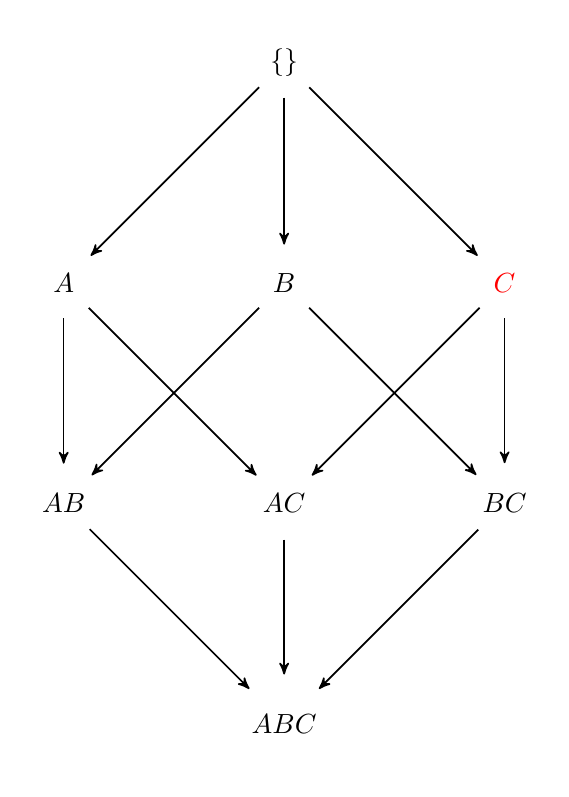
\begin{tikzpicture}[->,>=stealth',shorten >=1pt,auto,node distance=2.8cm,
                    semithick]
  \tikzstyle{every state}=[fill=white,draw=none,text=black]

  \node[state]         (Z)                    {$\{\}$};
  \node[state]         (B) [below  of=Z]      {$B$};
  \node[state]         (A) [left  of=B]       {$A$};
  \node[state]         (C) [right of=B]       {$\crouge{C}$};
  \node[state]		   (AB) [below of=A]      {$AB$};
  \node[state]		   (AC) [right of=AB]     {$AC$};
  \node[state]         (BC) [right of=AC]     {$BC$};
  \node[state] 		   (ABC) [below of=AC]    {$ABC$};
  

  \path (Z) edge              node {} (A)
            edge              node {} (B)
            edge			  node {} (C)
        (A) edge			  node {} (AB)
        	edge			  node {} (AC)
        (B) edge			  node {} (AB)
        	edge			  node {} (BC)
        (C) edge 			  node {} (AC)
        	edge			  node {} (BC)
        (AB) edge 			  node {} (ABC)
        (AC) edge			  node {} (ABC)
        (BC) edge			  node {} (ABC);
\end{tikzpicture} }
\end{multicols}
\end{center}

Cette technique, beaucoup utilisé en fouille de données, a ses limites, quelques années plus tard vient les premiers algorithmes de machine learning qui de nos jours sont encore bien répandue, en voici une liste non exhaustif:

\begin{description}
\item[Gradient]: Pour un nuage de points, le but est de trouver une droite qui minimise la distance (sur l'axe Y) entre celle ci et chaque  points du nuage.
\item[Kmeans]: Pour chaque sample du dataset, le but est de former des groupes de samples qui se ressemble le plus.
\end{description}

Ci dessus, deux modèle du machines learning, le Gradient est un modèle dit \textit{Supervisé} et le Kmeans est dit \textit{Non Supervisé}. La différence entre les deux modèle et simple, soit un dataset possédant une colonne nommé \textit{Étiquette} (ou Class en anglais) donne le résultat du sample concerné, il est donc facile pour un sample possédant une colonne Étiquette de connaitre son appartenance, on dit alors que le modèle est supervisé, pour un modèle non supervisé, nous ne connaissons pas les étiquettes des samples.\\
\pagebreak

\section{Algorithmes d'apprentissage}

De nos jours il existe une tonne d'algorithme d'apprentissage, tout ont plus ou moins leurs utilité, avantage, faiblesse, d'où le fait que pour le data scientiste doit essayer un peu tout les algorithmes et de juger de leurs efficacité via les résultats donnée. Bien-sûr si un Gradient suffit pourquoi vouloir utiliser un réseaux de neurones.\\
En voici une liste non exhaustive utilisé lors du stage à des fins de teste (via la librairie sci-kit-learn de python):

\begin{description}
\item[Support Vector Machine]: Le support vector machines cherche un hyperplan (de couleur noir) pouvant départager des classes,
Il en existe une infinité d'hyperplan qui peuvent les départager, donc introduisons un autre concept, celui de 
l'hyperplan qui maximise la séparation entre les deux classes (les droites $\corange{Oranges}$ appelé $Margin$.\\
\cshape{0.5}{
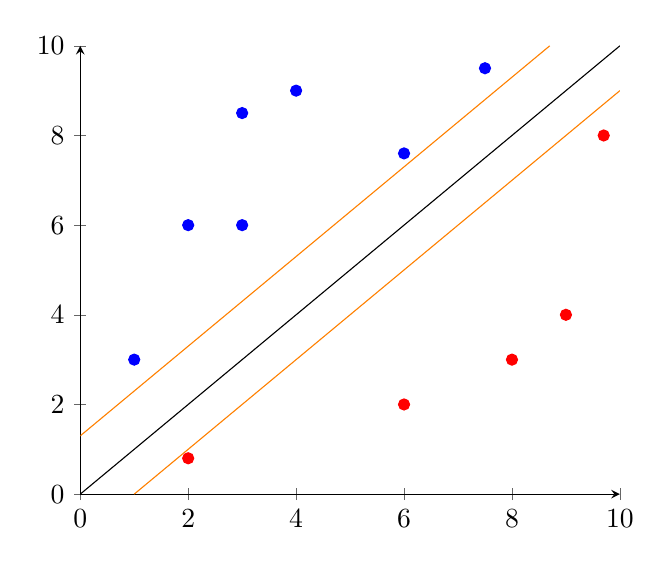
\begin{tikzpicture}
  \begin{axis} [
      axis lines = left,
      xmin       = 0,
      ymin       = 0,
    ]
    \addplot [color=black] coordinates {(0,0)(10,10)};
    \addplot [color=orange] coordinates {(0,1.3)(8.7,10) };
    \addplot [color=orange] coordinates {(1,0)(10,9) };
    \addplot [only marks, mark=*, color=blue] coordinates {(2,6)(1,3)(6,7.6)(3,8.5)(7.5,9.5)(4,9)(3,6)};
    \addplot [only marks, mark=*, color=red]  coordinates {(2,0.8)(6,2)(9,4)(9.7,8)(8,3)};
  \end{axis}
\end{tikzpicture}
}

\item[Decision Tree]: Un arbre de décision est une suite de nœuds relié par au moins une arrête, on emprunte une arrête par rapport à la décision qui est à prendre via le nœuds courant. L'ordre des nœuds est choisis selon des critères (les trois les plus utilisé sont \textit{Entropy}, \textit{Information grain} et \textit{Gini}), ces trois critères de sélection appliqué au même dataset peut donner un arbre diffèrent. Une feuille d'arbre est un nœuds n'ayant aucun fils, les étiquettes des prédictions s'y trouve.
\cshape{0.5}{
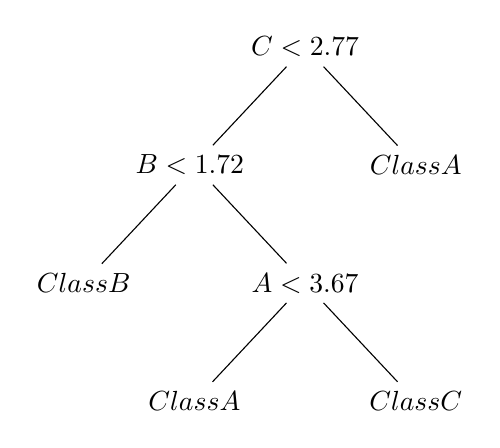
\begin{tikzpicture}[sibling distance=8em,
  every node/.style = {scale=1,
    draw=none, align=center}]]
  \node {$C < 2.77$}
 	  child { node {$B < 1.72$ }
 	    child { node {$Class B$}}
 	    child { node {$A < 3.67$}
 	      child { node {$Class A$}
 	      }
 	      child { node {$Class C$} }
 	    }
 	  }
 	  child { node {$Class A$} }
    ;
\end{tikzpicture}
}
\end{description}

\pagebreak
Traiter les samples de type numérique donne beaucoup de possibilités de traiter un problème.\\
L'évolution a fait que de plus de données sont de type textuel, pour des dates et durées, le problème reste simple à résoudre, pour une suite de mots fini, il suffit de les énumérer, mais pour les données du langage naturel?\\
\linebreak

\section{Langage naturel}

Un texte peu être long ou court, contenant des liens, des caractères spéciaux, on ne peut pas utiliser lancer un algorithme comme ci dessus sur des textes et en espérer en tirer de bon résultats, plusieurs étapes sont nécessaire pour pouvoir utiliser des algorithmes qui travaillent avec des textes. 

\subsection{Nettoyage des données}

Le français est un langage riche en dérivé de lettres notamment pour ses caractères accentués, le premier travail est de réduire l'espace des caractères en éliminent par exemple les majuscules et les remplacer par des minuscules, éliminer la ponctuation, puis normaliser les accents. Nous pouvons obtenir un texte comme suite:
\\
\sepline\\
Bonjour, je viens parce-que j'ai une fuite d'eau sur mon plafond, j'ai déjà prit contact avec une entreprise pour ses réparations mais elle n'a pas donné suite.\\
\sepline\\
bonjour je viens parce que j ai une fuite d eau sur mon plafond, j ai deja prit contact avec une entreprise pour ses reparations mais elle n a pas donne suite\\
\sepline\\



\chapter{Contexte du Stage}
Dans ce chapitre, nous allons introduire l'entreprise d'accueil, le cadre de travail, une petite description des outils utilisé (seulement les outils qui ne méritent pas une trop grande intention), une descriptions plus approfondit ce certains outils dans le chapitre suivant, de la méthodologie de travail utilisé puis le sujet de la mission.
\pagebreak

\section{Présentation de l'entreprise}
Crée en 2005 par deux frères, l'entreprise $\_$ maintenant basé à $\_$, Étant une société de service, proposant à ses collaborateurs une solution humaine de personnes maîtrisant leurs sujets le tout pour donner une équipe opérationnel pour toutes réalisation de projets.\linebreak
Les domaines de compétences vont du classique Java, passant par des standards comme php, docker vers l'incontournable Python. Aujourd'hui nous comptons environs une quarantaine de prestataire de talent couvrant les grand standards du monde numérique dans le quel nous baignons.\linebreak

\section{Présentation de la mission}
La demande du client est de pouvoir avoir un service pouvant traiter les demandes des clients dans les heurs où le standard d'écoute n'est présent, avant ce projet, toutes les demandes passèrent dans la catégorie des astreintes. Notre Intelligence artificiel doit simuler une conversation normal tout en dirigent les questions posé par rapport à la problématique du client puis de décider si oui ou non la résultante de l'appelle sera une astreinte ou non.
\pagebreak

\section{Cadre de travail}
Le cadre de travail ce situer au Centre de service, dans un open-space assez spacieux, accompagné d'une petit cuisine, et de quelques sales de repos.\\
Les interactions se faisais soit par Chat écrit, par mail ou via les réunions presque hebdomadaire qui constituai une partie de la méthodologie agile au quel j'étais impliqué dans les projets.
Bien entendu, à ne pas oublier le Git de l'entreprise pour toutes les solutions de travail collaboratif.

\section{Outils de travail}
Je vais énumérer les outils utilisé qui ont soit servit à l'analyse des data, la construction des jeux de données, les technologies vu qui n'ont pas étais implémenté et les algorithmes qui ont était testé.\\
\linebreak
\begin{description}
\item[DataIku]: Un logiciel qui permet le traitement de données de masse via de nombreux algorithmes présent par défaut allant de la simple transformation de dates (transformation, extraction, opération, ...) en traitement du langage naturel (lower, normalise, tokenise, ...), quelques algorithmes provenant du module python \textit{scikit-learn} comme les régressions logistique, foret d'isolation ou un réseau neuronal permettant d'avoir une prévisualisation des grands algorithmes dans une seul fenêtre, ceci a donné lieu à une simplification du choix des algorithmes pour les prédictions.
\item[DeepSpeech]: une solution de transformation de la voix en texte proposé par la fondation Mozilla utilisant la librairie python \textit{Tensorflow}.
\item[Spacy]: Une librairie python traitent des motifs du langage naturel, l'extraction de sous chaîne utilise la notion de \textit{POST-tagging} et ainsi découper le texte en une class d'éléments tel que son genre, son lien avec le reste de la phrase, ...
\item[Apriori]: un algorithme de fouille de donné qui se base sur la notion d'\textit{itemset}, cette algorithme a était abandonné même si dans un premier temps donnait de meilleurs résultats que le réseaux bayésiens naïf lors de la partie ontologie.
\end{description}

\pagebreak

\part{Un chatbot}

Le but initiale d'un chatbot est un agent pouvant dialoguer avec un utilisateur dans un certain contexte, un contexte est un ensemble de mots donnant lieu à un langage.\linebreak
Un modèle très basique de chatbot est une simplement un programme qui récupère clavier de l'utilisateur puis affiche une réponse formaté, les chatbot basique sont pas aussi intelligent, le contexte de la conversation a besoin d'être conservé pour pouvoir donner un meilleur sens et une interaction bien plus intéressante avec l'utilisateur.\linebreak
\\
Pour qu'un chatbot soit intéressant, celui-ci doit savoir de quoi on parle et savoir donner des réponses pertinentes, sans compter sur la qualité des réponses qui doivent être humainement compréhensible.\linebreak
\linebreak
Dans cette partie, nous allons voir les technologies utilisées, les algorithmes utilisées, des papiers théoriques et pratiques des recherches sur certains algorithmes utilisées et l'assemblage de tout ses composant pour aboutir à un prototype du projet final.

\chapter{Le langage naturelle}

Le langage naturelle n'est pas aussi facile à interprété que une série de valeurs pour les algorithmes de machine learning, c'est pour cela que pour gérer le langage naturelle, nous avons d'autres algorithmes que ce cité ci dessus.
Nous parlerons de \textit{Sequence To Sequence}, \textit{Long Short Term Memory},  \textit{Conditional Random Field}, \textit{Named Entities Recognition} ou de réseaux bayésiens naïf.\\

\pagebreak
\section{Les réseaux bayésiens naif}

C'est la première référence que nous avons quand on cherche dans le registre du travail avec les chaines textuelles.\\
L'idée du réseau bayésiens naïf est de représenter un ensemble de documents en une liste de fréquences de pairs $(w, |w|)$, w était un mot dans le langage des documents concerné, pour chaque labels, nous allons construire un modèle de probabilité via la formule suivante:
\formula{$P(X|Y=y)$}
Pour classifier un document, nous allons utilisé la formule ci dessous et retirer le meilleur résultat en tant que prédiction:
\formula{$ pred = P(X|y) * P(y)$}

D'après le module \textit{Scikit-Learn}, la variante Multinomial se démarque des autres variantes pour des raison de fonctionnement, la où les autres variantes demandent des cardinaux des mots, le multinomial fonctionne avec l'algorithme nommé \textit{TF-IDF}, cette algorithme sera introduit sous peu.\linebreak
\linebreak
Prenons ses deux corpus suivant, extrait de wikipedia. (le label de chaque corpus est représenté par un mot en gras):\\
\begin{description}
\item[Pomme]: La pomme est un fruit comestible à pépins d'un goût sucré et acidulé et à la propriété plus ou moins astringente selon les variétés. D'un point de vue botanique, il s'agit d'un faux-fruit. Elle est produite par les pommiers.
\item[Automobile]: Le terme populaire automobile désigne un véhicule à roues mû par un moteur et destiné au transport terrestre de personnes et de biens.
\end{description}

\pagebreak

La procédure d'apprentissage par Multinomial demande deux traitement sur la donnée, la première est nommé $Tokenization$ et la seconde $Frequencies$:\\
\begin{description}
\item[$Tokenization$]: Pour une chaine textuelle, nous allons supprimer tout les mots dit $stopwords$ comme $'le','la','ces',...$ des mots qui n'ont aucun impacte sur le sens général du texte, si on applique à $\textbf{Automobile}$ ceci donnerai: 
\begin{description}
\item[] terme populaire automobile désigne véhicule roues moteur destiné transport terrestre personnes.
\end{description}

\item[$Frequencies$]: Pour chaque mots présent dans le texte courant, nous allons lui associer un un dans son vecteur, la valeur vide étant zero. Pour que le tableau ne soit pas très large, nous allons prendre ses deux textes suivant: 
\begin{description}
\item[1:] gare train gauche gauche magasin
\item[2:] chaussures rangé haut magasin
\end{description}
Ce qui donne:\\\\
\begin{tabular}{c|c|c|c|c|c|c|c}
$-$ & chaussures & gare & gauche & haut & magasin & rangé & train\\
\hline
1: & 0 & 1 & 2 & 0 & 1 & 0 & 1\\
2: & 1 & 0 & 0 & 1 & 1 & 1 & 0\\
\end{tabular}
\end{description}

\ \linebreak
Pour avoir une implémentation complète venant de $scikit-learn$, la $tokenization$ sera décrit par l'algorithme $CountVectorizer$ et la $Frequencies$ par $TF-idf$.\\
\pagebreak

\section{Conditional Random Field}
Un autre modèle statistique, mais qui cette fois ne s'arrête pas à un simple encodage des variables, mais prend aussi en compte les variables voisines, pour correctement illustrer, prenons trois mots d'une phrase, comme $"pour$ $correctement$ $illustrer"$, et prenons le mot $"correctement"$, ce mot sera inséré dans une structure de données ayant comme champs:
\begin{description}
\item[lower]: le mot en minuscule (donc $"correctement"$)
\item[digit]: un boolean disant si le mot est un nombre ou pas
\item[title]: si ce mot est un titre (sous la forme capitalisé)
\item[trois champs -1]: qui lui contient les trois champs du dessus mais avec le mot $n-1$ 
\item[trois champs +1]: qui lui contient les trois champs du dessus mais avec le mot $n+1$ 
\end{description}

Ce modèle largement utilisé lorsque qu'on veut traiter le langage naturelle donne d'assez bon résultats.\\
\linebreak
Pour appuyer la qualité des résultats, en 2018, l'entreprise Google a développé un algorithme nommé \textbf{BERT} un outils de pré traitement du langage naturelle qui a significativement amélioré les algorithmes de traitement du langage naturelle. Dans le cadre du CRF nous utilisons le mot $n+/-1$ pour $n$, la où \textbf{BERT} prend en compte aussi les mots $n+/-2$, mais ce n'est pas tout, quand l'algorithme devait être testé, celui-ci devait deviner un mot en index $n$ de la phrase en ayant que ses 4 mots, les résultats était correct sans plus, donc en amélioration ils ont finalement laisser le pouvoir à l'algorithme de pouvoir lire la phrase en entier du sens normal (de gauche à droite) et aussi de lire la phrase de droite à gauche, ainsi de considérablement augmenter la précision des réponses.
\chapter{l'api de prédiction}
La brique du chatbot étant fini, reste la partie Machine Learning, j'ai décidé de séparer le chatbot des programmes d'intelligence artificielle et de placer tous les programmes dans une API qui est obtenable via requêtes \textit{REST}, ainsi, l'implémentation du projet se fait beaucoup plus facilement, d'un coté tous les programmes de prédictions et de l'autre le chatbot.\\
Les requêtes à l'api de Machine Learning se fait dans les Actions du chatbot.\\
\linebreak
Pour aboutir à un chatbot qui répond plutôt bien aux attentes des utilisateurs, nous devons extraire la nature du problème ($nature\_probleme$) les équipements concernés (comme les murs, fenêtres, grillage) ($equipement$) et les demandes techniques (une réclamation, renseignement, incident)  ($demande\_technique$).

\pagebreak
\section{Les ontologies}
Une ontologie est un ensemble de concepts qui donnent un sens à un groupe de mots, dans le chapitre précédant lors de l'introduction des slots, il y a eu une petite notion d'ontologie, dans le fait que pour une phrase on extrait des mots pour les associer à des slots.\\
Mais l'implémentation de la déduction des variables demandées ($nature\_probleme$, $equipement$ et $demande\_technique$) est plus complexe. Pour un corpus de mots construits à partir de huit Gigabit de données clients et de quelques programmes d'automatisation de l'extraction et d'analyse fait par nous-même, nous avons pu construire les corpus comme suit:
\ \linebreak
\begin{lstlisting}
Mots_Clef_Demande_technique.csv

Clef,Synonyme
adaptation,"adaptation,adaptations,adapter,adapte,ajustement,ajustements,ajuster,..."
effraction,"effraction,pillage,piller,pille,vol ,voller,voleur,vol avec effraction, ..."
epave,"epave,epave,epaves,delabre,delabrer,ruine,debris, ..."
deratisation,"deratisation,deratisation,presence de rat,des rats"
...
\end{lstlisting}
\ \linebreak
Pour chaque mots dans les synonymes, on lui associe sa clef, ce qui donne par un exemple:
\ \linebreak
\begin{lstlisting}
str = "Il y a une epave de voiture qui est devant une maison abandonne depuis longtemps, ce matin des rats sont venue m'attaquer."
print(ontologies(demande_technique, str)
> ["epave", "deratisation"]
\end{lstlisting}
\ \linebreak

Nous avons résumé en ontologie la phrase donnée pour en obtenir une série de mot clefs, ainsi coupler avec un algorithme d'apprentissage travaillant sur les chaînes de caractères, comme un réseau bayésiens naïf nous obtenons le type de $demande\_technique$ associé à la phrase posé ci-dessus:

\pagebreak

\begin{lstlisting}
Demande_technique_train.csv

Class,Input
adaptation,"[adaptation]"
amenagement,"[voirie]"
maintenance,"[maintenance,reclamation]"
incident,"[degradation,garantie]"
reclamation,"[change,degradation,reclamation]"
occupation_vide,"[epave]"
\end{lstlisting}

Nous comptons respectivement pour les trois ontologies ($nature\_probleme$, $equipement$ et $demande\_technique$), au moins deux cents synonymes (par fichier) pour respectivement 30, 52 et 23 clefs pour les fichiers des mots clefs et respectivement 975, 1242 et 156 lignes d'apprentissage pour l'algorithme de réseau bayésiens naïf.\\
A l'aide d'un de nos programmes, nous avons pu faire un estimateur sur le pouvoir de notre ontologie, nous avons semi automatisé la classification des huit Gigabit de transcrits et nous avons appelé l'entièreté des phrases utilises (donc des phrases autre que "oui","bonjour", "au revoir"...) sur notre api, les résultats pour $demande\_technique$ ne sont pas mauvais

\begin{lstlisting}
comportement_invervenant: OK:    0 | NOK:    0 | TOTAL:    0 | RATIO:0.00000
                        securiter: OK:    1 | NOK:    1 | TOTAL:    2 | RATIO:0.50000
                  contestation: OK:  127 | NOK:   85 | TOTAL:  212 | RATIO:0.59906
                amenagement: OK:  373 | NOK:  154 | TOTAL:  527 | RATIO:0.70778
                    abandonne: OK:   68 | NOK:   27 | TOTAL:   95 | RATIO:0.71579
                 maintenance: OK:  130 | NOK:   42 | TOTAL:  172 | RATIO:0.75581
                  reclamation: OK: 2126 | NOK:  678 | TOTAL: 2804 | RATIO:0.75820
                     adaptation: OK:   70 | NOK:   12 | TOTAL:   82 | RATIO:0.85366
             eclairage_collectif: OK:   51 | NOK:    8 | TOTAL:   59 | RATIO:0.86441
                            epave: OK:   14 | NOK:    2 | TOTAL:   16 | RATIO:0.87500
                       effraction: OK:   27 | NOK:    3 | TOTAL:   30 | RATIO:0.90000
                           voirie: OK:  411 | NOK:   35 | TOTAL:  446 | RATIO:0.92152
                   intervention: OK:  743 | NOK:   55 | TOTAL:  798 | RATIO:0.93108
                    degradation: OK:  282 | NOK:    8 | TOTAL:  290 | RATIO:0.97241
                    information: OK: 4999 | NOK:  107 | TOTAL: 5106 | RATIO:0.97904
                          change: OK:  691 | NOK:   10 | TOTAL:  701 | RATIO:0.98573
                        garantie: OK:  530 | NOK:    7 | TOTAL:  537 | RATIO:0.98696
                        incident: OK:  403 | NOK:    3 | TOTAL:  406 | RATIO:0.99261
                deinsectisation: OK:    1 | NOK:    0 | TOTAL:    1 | RATIO:1.00000
                     non_resolu: OK:    2 | NOK:    0 | TOTAL:    2 | RATIO:1.00000
                   amelioration: OK:   21 | NOK:    0 | TOTAL:   21 | RATIO:1.00000
                            squat: OK:    5 | NOK:    0 | TOTAL:    5 | RATIO:1.00000
                   deratisation: OK:   16 | NOK:    0 | TOTAL:   16 | RATIO:1.00000
\end{lstlisting}
\pagebreak

\section{Les algorithmes annexes}

Dans notre API, je viens d'expliquer la brique la plus importante, mais je voudrais aussi évoquer les autres \textit{end-points} qui ont leurs intérêts dans la construction du projet:

\begin{description}
\item[Normalizer]: traitent toutes chaînes avant tokenisation en enlevant les url, les caractères spéciaux, les accents et les majuscules.
\item[Tokenizer]: Qui pour un corpus de mots clefs, (voir un exemple ci-dessus) transforme la phrase précédemment normalisé en un ensemble de mots clefs
\item[un\_une]: qui pour un mot, donne sont genre ("un" ou "une"), utilisant un algorithme de réseau bayésiens naïf.
\item[un\_des]: qui pour un mot, prédit son article (du,de la,des,l') afin de construire des phrases le plus humainement compréhensible.
\item[astreinte]: qui pour un motif, un équipement et une nature problème précédemment prédit va prédire si une astreinte est requit pour le problème.
\item[ner]: Qui pour une phrase du client retourne que la partie intéressante (voir dans la section NER au-dessus)
\formula{"J'ai une fuite dans ma salle de bain et mes enfants jouent dans le jardin"}
\formula{"une fuite dans ma salle de bain"}
\item[ner\_conjugate]: qui pour une phrase extraite depuis le NER va changer les mots donnant l’impression que le bot répond normalement à une phrase:
\formula{"une fuite dans ma salle de bain"}
\formula{"votre fuite dans votre salle de bain"}
\item[pos\_neg]: qui pour une réponse donnée sous forme d'une phrase, prédit si la réponse est positif ou négatif.
\end{description}



\chapter{Fonctionnement de l'application}
Toutes les pièces du puzzle ont été introduit, il ne manque plus qu'a les assembler pour construire le chatbot. Comme expliqué ci-dessus, les algorithmes de prédictions seront tous dans l'api via le protocole REST, le chatbot sera équipé d'une brique NLU et CORE, un formulaire d'action qui va s'occuper de remplir les slots et appeler l'api de prédiction.\linebreak
Dans ce chapitre nous allons voir le bot en action.

Voici une interaction avec le chatbot:

\begin{description}
\item[user]: bonjour
\item[bot]: Bonjour je suis marie, quelle est votre soucie
\item[user]: voilà je vous appel car ma chaudière est en panne
\item[bot]: Parler moi plus en détail de votre chaudière qui est en panne, si vous en avait
\item[user]: elle ne fonctionne plus quand je l'allume
\item[bot]: Je vais faire monter l'information au service concerné qui vous rappellera
\item[bot]: au revoir.	
\end{description}

Le chatbot possède aussi un port serveur, les appelles se font via le protocole REST entièrement en \textit{POST}.\linebreak
Le premier souci du chatbot c'est que nous ne pouvons pas faire passer à travers le chatbot une interaction entre deux clients sans que celui-ci ne consomme les données, donc il a fallu un programme fessant office de routeur pour les conversations de l'utilisateur, soit le schéma suivant:

\begin{center}
\includegraphics[scale=0.9]{img/plans.jpg}
\end{center}

Lors de la phase de développement du projet, le programme routeur était un programme python, qui attendait un certain paquet provenant du bot pour pouvoir changer l'url d’envois des données vers un service client. Une fonctionnalité en plus est que le bot à un annuaire (noté par la base de données \textit{Human Chat Links db} qui redirige le client vers tel endpoint de telle adresse de tel service.\linebreak

\section{Implémentations futures}

Dans ce qu'il reste du projet, nous devons brancher le chatbot sur une interface pouvant être compatible avec un téléphone, donc nous devons avoir une brique transformant la voix en texte et inversement, nous allons utiliser \textit{DeepSpeech} la librairie de Mozilla qui va nous permettre via des algorithmes Tensorflow et Seq2Seq de générer un modèle répondant à nos besoins.\linebreak

\chapter{Conclusion}

Ce fut un stage riche en découverte, une bonne continuation des cours de machines learning proposé à la faculté, un branchement plus que parfait. Lorsque qu'à la fac nous apprenons les bases du machine learning, de la fouille de données, et quelques implémentations avec des datasets plus orienté numérique, le stage s'est directement enchaîné avec du travail sur le langage naturelle.\linebreak
la méthodologie agile m'as permis de me donner des objectifs à réaliser dans des délai autre que la deadline du projet.\linebreak
J'ai gagné en compétence dans l'art de la fouille de données et dans l'analyse de données en ayant travaillé avec des donnée clients car qui a donné un vrai terrain d'apprentissage du métier de \textit{Data Analyste} dans la vie professionnel.


\part{Références}

\newcommand{\reff}[2]{\item[\textbf{\textit{#1}}]: \textit{#2}}

\begin{description}
\reff{Rasa}{$https://rasa.com/docs/$}
\reff{Spacy}{$https://spacy.io/models$}
\reff{SkLearn}{$https://scikit-learn.org/stable/modules/classes.html$}
\reff{Seq2Seq}{$https://google.github.io/seq2seq/nmt/$}
\reff{LSTM}{$https://en.wikipedia.org/wiki/Long\_short-term\_memory$}
\reff{DeepSpeech}{$https://github.com/mozilla/DeepSpeech$}
\reff{Seq2Seq text summarization}{$https://github.com/dongjun-Lee/text-summarization-tensorflow$}
\reff{Seq2Seq text to speech}{$https://arxiv.org/pdf/1903.07398.pdf$}
\reff{Pos Tagging}{$https://spacy.io/usage/linguistic-features\#pos-tagging$}
\reff{CRF Suite}{$https://sklearn-crfsuite.readthedocs.io/en/latest/$}
\reff{Pomme}{$https://fr.wikipedia.org/wiki/Pomme$}
\reff{Automobile}{$https://fr.wikipedia.org/wiki/Automobile$}
\end{description}

	
	

\pagebreak
\end{document}


